% \VignetteEngine{knitr::knitr}
% \VignetteIndexEntry{04. Bioconductor for Sequence Analysis -- slides}

\documentclass[xcolor=dvipsnames]{beamer}\usepackage[]{graphicx}\usepackage[]{color}
%% maxwidth is the original width if it is less than linewidth
%% otherwise use linewidth (to make sure the graphics do not exceed the margin)
\makeatletter
\def\maxwidth{ %
  \ifdim\Gin@nat@width>\linewidth
    \linewidth
  \else
    \Gin@nat@width
  \fi
}
\makeatother

\definecolor{fgcolor}{rgb}{0.345, 0.345, 0.345}
\newcommand{\hlnum}[1]{\textcolor[rgb]{0.686,0.059,0.569}{#1}}%
\newcommand{\hlstr}[1]{\textcolor[rgb]{0.192,0.494,0.8}{#1}}%
\newcommand{\hlcom}[1]{\textcolor[rgb]{0.678,0.584,0.686}{\textit{#1}}}%
\newcommand{\hlopt}[1]{\textcolor[rgb]{0,0,0}{#1}}%
\newcommand{\hlstd}[1]{\textcolor[rgb]{0.345,0.345,0.345}{#1}}%
\newcommand{\hlkwa}[1]{\textcolor[rgb]{0.161,0.373,0.58}{\textbf{#1}}}%
\newcommand{\hlkwb}[1]{\textcolor[rgb]{0.69,0.353,0.396}{#1}}%
\newcommand{\hlkwc}[1]{\textcolor[rgb]{0.333,0.667,0.333}{#1}}%
\newcommand{\hlkwd}[1]{\textcolor[rgb]{0.737,0.353,0.396}{\textbf{#1}}}%

\usepackage{framed}
\makeatletter
\newenvironment{kframe}{%
 \def\at@end@of@kframe{}%
 \ifinner\ifhmode%
  \def\at@end@of@kframe{\end{minipage}}%
  \begin{minipage}{\columnwidth}%
 \fi\fi%
 \def\FrameCommand##1{\hskip\@totalleftmargin \hskip-\fboxsep
 \colorbox{shadecolor}{##1}\hskip-\fboxsep
     % There is no \\@totalrightmargin, so:
     \hskip-\linewidth \hskip-\@totalleftmargin \hskip\columnwidth}%
 \MakeFramed {\advance\hsize-\width
   \@totalleftmargin\z@ \linewidth\hsize
   \@setminipage}}%
 {\par\unskip\endMakeFramed%
 \at@end@of@kframe}
\makeatother

\definecolor{shadecolor}{rgb}{.97, .97, .97}
\definecolor{messagecolor}{rgb}{0, 0, 0}
\definecolor{warningcolor}{rgb}{1, 0, 1}
\definecolor{errorcolor}{rgb}{1, 0, 0}
\newenvironment{knitrout}{}{} % an empty environment to be redefined in TeX

\usepackage{alltt}

\usepackage{BioconductorSlides}
\hypersetup{colorlinks,linkcolor=,urlcolor=Blue}

\title{\Bioconductor{} for Sequence Analysis}
\author{Alex S\'anchez\footnote{Adapted from MArtin Morgan's slides}}
\IfFileExists{upquote.sty}{\usepackage{upquote}}{}
\begin{document}

\maketitle

\begin{frame}{Introduction: What is \Bioconductor{} good for?}
  \begin{itemize}
  \item Sequencing: RNA-seq, ChIP-seq, called variants, \ldots 
    \begin{itemize}
    \item Especially \emph{after} assembly / alignment
    \end{itemize}
  \item Annotation: genes, pathways, gene models (exons, transcripts,
    etc.), \ldots
  \item Microarrays: expression, copy number, SNPs, methylation, \ldots
  \item Flow cytometry, proteomics, image analysis, high-throughput
    screens, \ldots
  \end{itemize}
\end{frame}


\begin{frame}[fragile]{Sequencing: The \Biocpkg{ShortRead} package}
\begin{knitrout}
\definecolor{shadecolor}{rgb}{0.969, 0.969, 0.969}\color{fgcolor}\begin{kframe}
\begin{alltt}
\hlcom{## Use the 'ShortRead' package}
\hlkwd{library}\hlstd{(ShortRead)}
\hlcom{## Create an object to represent a sample from a file}
\hlstd{sampler} \hlkwb{<-} \hlkwd{FastqSampler}\hlstd{(}\hlstr{"ERR127302_1.fastq.gz"}\hlstd{)}
\hlcom{## Apply a method to yield a random sample}
\hlstd{fq} \hlkwb{<-} \hlkwd{yield}\hlstd{(sampler)}
\hlcom{## Access sequences of sampled reads using `sread()`}
\hlcom{## Summarize nucleotide use by cycle}
\hlcom{## 'abc' is a nucleotide x cycle matrix of counts}
\hlstd{abc} \hlkwb{<-} \hlkwd{alphabetByCycle}\hlstd{(}\hlkwd{sread}\hlstd{(fq))}
\hlcom{## Subset of interesting nucleotides}
\hlstd{abc} \hlkwb{<-} \hlstd{abc[}\hlkwd{c}\hlstd{(}\hlstr{"A"}\hlstd{,} \hlstr{"C"}\hlstd{,} \hlstr{"G"}\hlstd{,} \hlstr{"T"}\hlstd{,} \hlstr{"N"}\hlstd{),]}
\end{alltt}
\end{kframe}
\end{knitrout}
\end{frame}

\begin{frame}[fragile]{Sequencing: The \Biocpkg{ShortRead} package}
  \begin{columns}
    \column{.5\textwidth}
\begin{knitrout}
\definecolor{shadecolor}{rgb}{0.969, 0.969, 0.969}\color{fgcolor}\begin{kframe}
\begin{alltt}
\hlcom{## Create a plot from a}
\hlcom{## matrix}
\hlkwd{matplot}\hlstd{(}\hlkwd{t}\hlstd{(abc),} \hlkwc{type}\hlstd{=}\hlstr{"l"}\hlstd{,}
  \hlkwc{lty}\hlstd{=}\hlnum{1}\hlstd{,} \hlkwc{lwd}\hlstd{=}\hlnum{3}\hlstd{,}
  \hlkwc{xlab}\hlstd{=}\hlstr{"Cycle"}\hlstd{,}
  \hlkwc{ylab}\hlstd{=}\hlstr{"Count"}\hlstd{,}
  \hlkwc{cex.lab}\hlstd{=}\hlnum{2}\hlstd{)}
\hlcom{## Add a legend}
\hlkwd{legend}\hlstd{(}\hlstr{"topright"}\hlstd{,}
  \hlkwc{legend}\hlstd{=}\hlkwd{rownames}\hlstd{(abc),}
  \hlkwc{lty}\hlstd{=}\hlnum{1}\hlstd{,} \hlkwc{lwd}\hlstd{=}\hlnum{3}\hlstd{,} \hlkwc{col}\hlstd{=}\hlnum{1}\hlopt{:}\hlnum{5}\hlstd{,}
  \hlkwc{cex}\hlstd{=}\hlnum{1.8}\hlstd{)}
\end{alltt}
\end{kframe}
\end{knitrout}
    \column{.5\textwidth}
    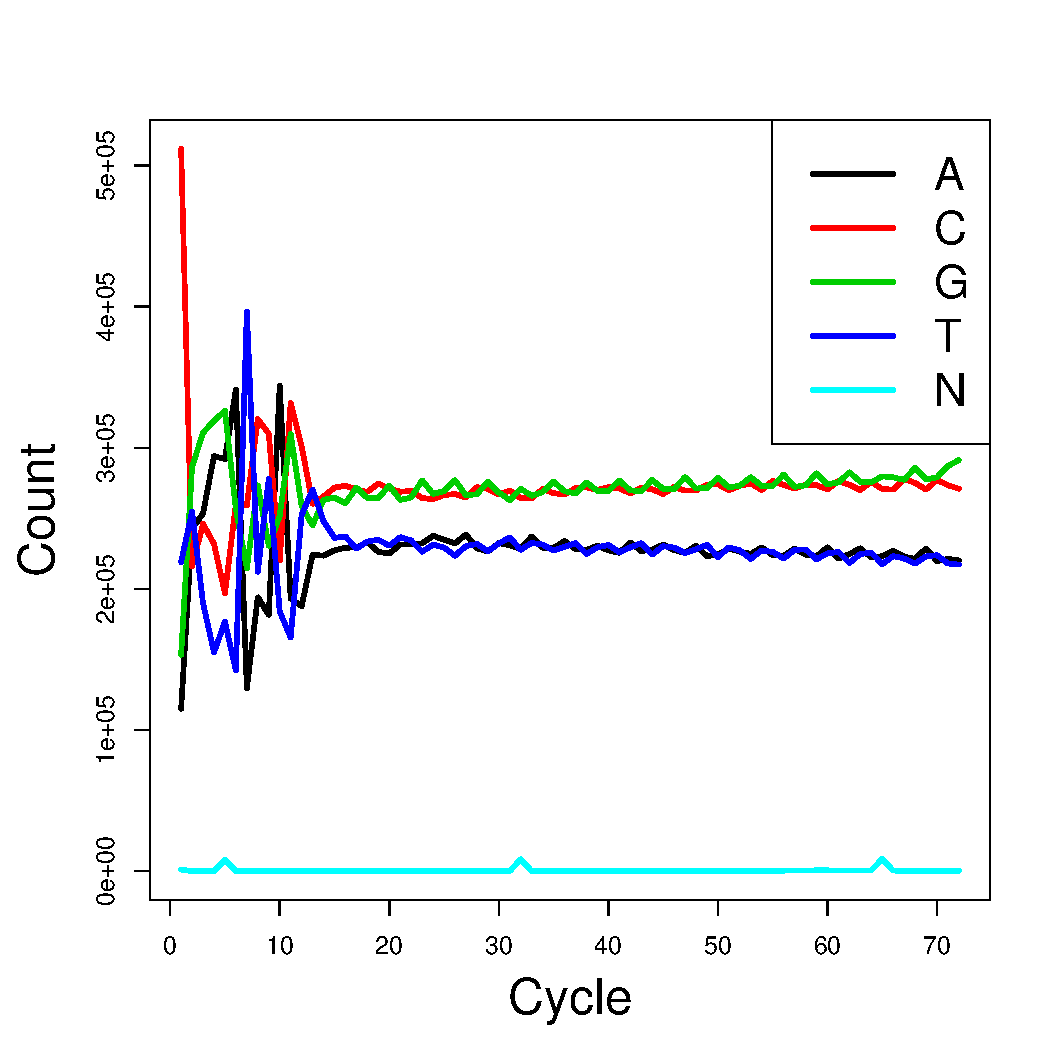
\includegraphics[width=\textwidth]{figures/abc}
  \end{columns}
\end{frame}

\begin{frame}{Sequencing: Essential packages and classes}
  \begin{itemize}
  \item \Biocpkg{Biostrings} and \Rclass{DNAStringSet}
  \item \Biocpkg{GenomicAlignments} and \Rclass{GAlignments}
  \item \Biocpkg{GenomicRanges} and \Rclass{GRanges}
  \item \Biocpkg{GenomicFeatures} and \Rclass{TranscriptDb}
  \item \Biocpkg{VariantAnnotation} and \Rclass{VCF}
  \item Input and output: \Biocpkg{rtracklayer} (WIG, BED, etc.),
    \Biocpkg{Rsamtools} (BAM), \Biocpkg{ShortRead} (FASTQ) file input
  \end{itemize}
\end{frame}

\section*{Sequencing: package tour}

\begin{frame}{Reads}
  \begin{description}
  \item[Data] Short reads and their qualities
  \item[Tasks] Input, quality assessment, summary, trimming, \ldots
  \item[Packages] \Biocpkg{ShortRead}, \Biocpkg{Biostrings}
  \item[Functions]
    \begin{itemize}
    \item \Rfunction{readFastq}, \Rfunction{FastqSampler},
      \Rfunction{FasqtStreamer}.
    \item \Rfunction{qa}, \Rfunction{report}.
    \item \Rfunction{alphabetFrequency}, \Rfunction{alphabetByCycle},
      \Rfunction{consensusMatrix}.
    \item \Rfunction{trimTails}, \Rfunction{trimLRPatterns},
      \Rfunction{matchPDict}, \ldots
    \end{itemize}
  \end{description}
\end{frame}

\begin{frame}{Alignments}
  \begin{description}
  \item[Data] BAM files of aligned reads
  \item[Tasks] Input, BAM file manipulation, pileups
  \item[Packages] \Biocpkg{GenomicAlignments}, \Biocpkg{Rsamtools}
    (also: \Biocpkg{GenomicRanges})
  \item[Functions]
    \begin{itemize}
    \item \Rfunction{readGAlignments}
    \item \Rfunction{BamFile}, \Rfunction{BamFileList}
    \item \Rfunction{scanBam}, \Rfunction{ScanBamParam} (select a
      subset of the BAM file)
    \item \Rfunction{asBam}, \Rfunction{sortBam},
      \Rfunction{indexBam}, \Rfunction{mergeBam},
      \Rfunction{filterBam}
    \item \Rfunction{BamSampler}, \Rfunction{applyPileups}
    \end{itemize}
  \end{description}
\end{frame}

\begin{frame}{Ranges}
  \begin{description}
  \item[Data] Genomic coordinates to represent data (e.g., aligned
    reads) or annotation (e.g., gene models).
  \item[Tasks] Input, counting, coverage, manipulation, \ldots
  \item[Packages] \Biocpkg{GenomicRanges}, \Biocpkg{IRanges}
  \item[Functions]
    \begin{itemize}
    \item \Rfunction{readGAlignments}, \Rfunction{readGAlignmentsList}
    \item Many intra-, inter-, and between-range manipulating, e.g.,
      \Rfunction{narrow}, \Rfunction{flank}, \Rfunction{shift},
      \Rfunction{intersect}, \Rfunction{findOverlaps},
      \Rfunction{countOverlaps}
    \end{itemize}
  \end{description}
\end{frame}

\begin{frame}{Variants}
  \begin{description}
  \item[Data] VCF (Variant Call Format) file
  \item[Tasks] Calling, input, summary, coding consequences
  \item[Packages] \Biocpkg{VariantTools} (linux only),
    \Biocpkg{VariantAnnotation}, \Biocpkg{ensemblVEP}
  \item[Functions]
    \begin{itemize}
    \item \Rfunction{tallyVariants}
    \item \Rfunction{readVcf}, \Rfunction{locateVariants},
      \Rfunction{predictCoding}
    \item Also: SIFT, PolyPhen data bases
    \end{itemize}
  \end{description}
\end{frame}

\begin{frame}{Annotations}
  \begin{description}
  \item[Data] Gene symbols or other identifiers
  \item[Tasks] Discover annotations associated with genes or symbols
  \item[Packages] \Biocpkg{AnnotationDbi} (\Rpackage{org.*},
    \Biocannopkg{GO.db}, \ldots), \Biocpkg{biomaRt}
  \item[Functions]
    \begin{itemize}
    \item Discovery: \Rfunction{columns}, \Rfunction{keytype},
      \Rfunction{keys}
    \item \Rfunction{select}, \Rfunction{merge}
    \item \Biocpkg{biomaRt}: \Rfunction{listMarts},
      \Rfunction{listDatasets}, \Rfunction{listAttributes},
      \Rfunction{listFilters}, \Rfunction{getBM}
    \end{itemize}
  \end{description}
\end{frame}

\begin{frame}{Features}
  \begin{description}
  \item[Data] Genomic coordinates
  \item[Tasks] Group exons by transcript or gene; discover transcript
    / gene identifier mappings
  \item[Packages] \Biocpkg{GenomicFeatures} and \Rpackage{TxDb.*}
    packages (also: \Biocpkg{rtracklayer})
  \item[Functions]
    \begin{itemize}
    \item \Rfunction{exonsBy}, \Rfunction{cdsBy}, \Rfunction{transcriptsBy}
    \item \Rfunction{select} (see Annotations, below)
    \item \Rfunction{makeTranscriptDb*}
    \end{itemize}
  \end{description}
\end{frame}

\begin{frame}{Genome annotations}
  \begin{description}
  \item[Data] FASTA, GTF, VCF, \ldots from internet resources
  \item[Tasks] Define regions of interests; incorporate known features
    (e.g., ENCODE marks, dbSNP variants) in work flows
  \item[Packages] \Biocpkg{AnnotationHub}
  \item[Functions]
    \begin{itemize}
    \item \Rfunction{AnnotationHub}, \Rfunction{filters}
    \item \Rfunction{metadata}, \Rcode{hub\$<tab>}
    \end{itemize}
  \end{description}
\end{frame}

\begin{frame}{Sequences}
  \begin{description}
  \item[Data] Whole-genome sequences
  \item[Tasks] View sequences, match position weight matricies, match
    patterns
  \item[Packages] \Biocpkg{Biostrings}, \Biocpkg{BSgenome}
  \item[Functions]
    \begin{itemize}
    \item \Rfunction{available.genomes}
    \item \Rcode{Hsapiens[["chr3"]]}, \Rfunction{getSeq}, \Rfunction{mask}
    \item \Rfunction{matchPWM}, \Rfunction{vcountPattern}, \ldots
    \item \Rfunction{forgeBSgenomeDataPkg}
    \end{itemize}
  \end{description}
\end{frame}

\begin{frame}{Import / export}
  \begin{description}
  \item[Data] Common text-based formats, \texttt{gff}, \texttt{wig},
    \texttt{bed}; UCSC tracks
  \item[Tasks] Import and export
  \item[Packages] \Biocpkg{rtracklayer}
  \item[Functions]
    \begin{itemize}
    \item \Rfunction{import}, \Rfunction{export}
    \item \Rfunction{browserSession}, \Rfunction{genome}
    \end{itemize}
  \end{description}
\end{frame}

\begin{frame}{And\ldots}
  
    Data representation: \Biocpkg{IRanges}, \Biocpkg{GenomicRanges},
    \Biocpkg{GenomicFeatures}, \Biocpkg{Biostrings},
    \Biocpkg{BSgenome}, \Biocpkg{girafe}.
    Input / output: \Biocpkg{ShortRead} (fastq), \Biocpkg{Rsamtools}
    (bam), \Biocpkg{rtracklayer} (gff, wig, bed),
    \Biocpkg{VariantAnnotation} (vcf), \Biocpkg{R453Plus1Toolbox}
    (454).
    Annotation: \Biocpkg{GenomicFeatures}, \Biocpkg{ChIPpeakAnno},
    \Biocpkg{VariantAnnotation}.
    Alignment: \Biocpkg{Rsubread}, \Biocpkg{Biostrings}.
    Visualization: \Biocpkg{ggbio}, \Biocpkg{Gviz}.
    Quality assessment: \Biocpkg{qrqc}, \Biocpkg{seqbias},
    \Biocpkg{ReQON}, \Biocpkg{htSeqTools}, \Biocpkg{TEQC},
    \Biocpkg{Rolexa}, \Biocpkg{ShortRead}.
    RNA-seq: \Biocpkg{BitSeq}, \Biocpkg{cqn}, \Biocpkg{cummeRbund},
    \Biocpkg{DESeq}, \Biocpkg{DEXSeq}, \Biocpkg{EDASeq},
    \Biocpkg{edgeR}, \Biocpkg{gage}, \Biocpkg{goseq},
    \Biocpkg{iASeq}, \Biocpkg{tweeDEseq}.
    ChIP-seq, etc.: \Biocpkg{BayesPeak}, \Biocpkg{baySeq},
    \Biocpkg{ChIPpeakAnno}, \Biocpkg{chipseq}, \Biocpkg{ChIPseqR},
    \Biocpkg{ChIPsim}, \Biocpkg{CSAR}, \Biocpkg{DiffBind},
    \Biocpkg{MEDIPS}, \Biocpkg{mosaics}, \Biocpkg{NarrowPeaks},
    \Biocpkg{nucleR}, \Biocpkg{PICS}, \Biocpkg{PING},
    \Biocpkg{REDseq}, \Biocpkg{Repitools}, \Biocpkg{TSSi}.
    Motifs: \Biocpkg{BCRANK}, \Biocpkg{cosmo}, \Biocpkg{cosmoGUI},
    \Biocpkg{MotIV}, \Biocpkg{seqLogo}, \Biocpkg{rGADEM}.
    3C, etc.: \Biocpkg{HiTC}, \Biocpkg{r3Cseq}.
    Copy number: \Biocpkg{cn.mops}, \Biocpkg{CNAnorm},
    \Biocpkg{exomeCopy}, \Biocpkg{seqmentSeq}.
    Microbiome: \Biocpkg{phyloseq}, \Biocpkg{DirichletMultinomial},
    \Biocpkg{clstutils}, \Biocpkg{manta}, \Biocpkg{mcaGUI}.
    Work flows: \Biocpkg{ArrayExpressHTS}, \Biocpkg{Genominator},
    \Biocpkg{easyRNASeq}, \Biocpkg{oneChannelGUI},
    \Biocpkg{rnaSeqMap}.
    Database: \Biocpkg{SRAdb}. \ldots
\end{frame}

\end{document}
